
\section{chapter over view}
\begin{itemize}

\item to assess the accuracy of current neural modelling work we explored:
\item variance in models
\item variance in experiments,  
\item variance in the combined set of models and experiments.


\end{itemize}


\title{Cortical Model and Cortical Experiment Agreement}
    % combine this discussion with model repurposing discussion.
Models and Data can agree and disagree in many different ways, therefore we would like to identify important sources of model/data disagreement. Better awareness of model/data disagreement informs a related question: "In  cortical neuron models which segmented pieces of a voltage recording waveform should the optimizer act on?"

\section{Features} Consider a voltage recording at the location of the membrane of a neuron. Teams of researchers have already segmented voltage recordings into labelled sections, each section has a classification that is based on the shape of waveform in a limited region. Rather than specifying by name each measurement it is often useful to refer collectively to these measurable shapes as "features". In multivariate analysis I look at hundreds of these waveform features. 

Specifically below, I describe some neuronal model features that agreed well with experiments, and some features that disagreed less well.
%\end{tcolorbox}
\begin{figure}    
\begin{center}

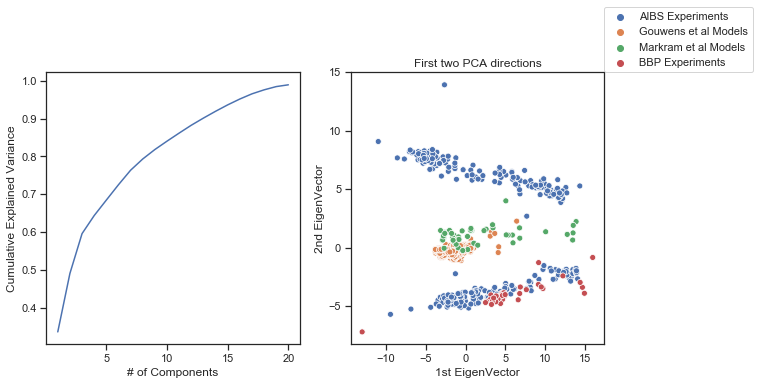
\includegraphics[width=0.7\linewidth]{figures/cortical_model_data_agreement_52_1.png}
\end{center}
\end{figure}    
\begin{figure}    
\begin{center}
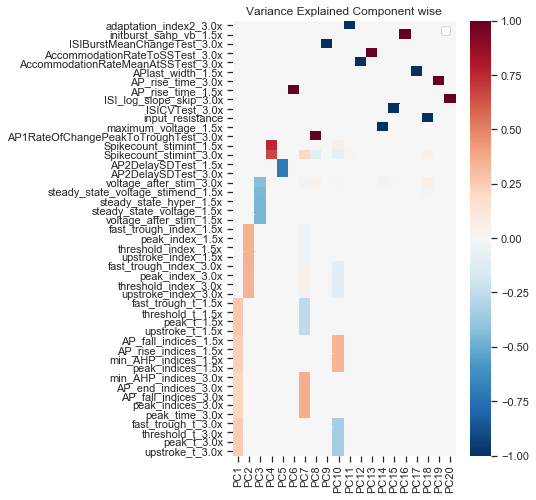
\includegraphics[width=0.7\linewidth]{../figures/cortical_model_data_agreement_54_1.png}
\end{center}
\end{figure}    

\section{sources of disagreement}
\begin{itemize}
    \item upstroke\_t\_1.5x allen feature
    \item  peak\_t\_1.5x allen feature
    \item threshold\_t\_1.5x allen feature
    \item fast\_trough\_t\_1.5x allen feature
    \item fast\_trough\_t\_3.0x allen feature
    \item upstroke\_t\_3.0x allen feature
    \item peak\_t\_3.0x allen feature
    \item threshold\_t\_3.0x allen feature
    \item peak\_indices\_1.5x efel feature
    \item min\_AHP\_indices\_1.5x efel feature
\end{itemize}



\section{Features that disagree} 
\begin{itemize}

    \item fast\_trough\_index\_1.5x allen feature
    \item peak\_index\_1.5x allen feature
    \item upstroke\_index\_1.5x allen feature
    \item threshold\_index\_1.5x allen feature
    \item fast\_trough\_index\_3.0x allen feature
    \item peak\_index\_3.0x allen feature
    \item upstroke\_index\_3.0x allen feature
    \item threshold\_index\_3.0x allen feature
\end{itemize}


